\documentclass[12pt]{article}
\usepackage{geometry}
\usepackage{graphicx}
\usepackage{tikz}
\usepackage{booktabs}
\usepackage{array}
\usepackage{multirow}
\usepackage{makecell}
\usepackage{amsmath}
\usepackage{float}
\usetikzlibrary{decorations.text}
\geometry{margin=1in}
\title{Product Requirements Document (PRD):\newline Detection of U.S. Surface Ships by Chinese UAVs and Fishing Boats}
\author{Rob Kieneker \\ Matthew Cancian}
\date{August 8, 2025}

\begin{document}
\maketitle

\section{Purpose}
This program calculates the likelihood and timing of Chinese UAVs and fishing boats detecting U.S. surface ships operating between 3,500--4,000 km from the coast of China. The simulation uses agent-based modeling and Monte Carlo methods, with outputs summarized in a detection time matrix for various force compositions and patrol densities.

\section{Scope}
\begin{itemize}
	\item Simulate detection of U.S. ships by Chinese UAVs/fishing boats in a large maritime area.
	\item Model three U.S. formations: single destroyer, multiple destroyers, and multiple destroyers with an aircraft carrier.
	\item Vary Chinese patrol density: 10\%, 25\%, 50\%, 75\% of available UAVs/fishing boats.
	\item Output: Median time to detection for each scenario, summarized in a matrix.
	\item No combat; only detection/observation events.
\end{itemize}

\section{Area of Interest}
The area is defined by a baseline of 600 km, extending outwards at 120 degrees on both sides, forming a wide sector that reaches up to 4,500 km from the baseline. U.S. ships enter from the far edge (3,500--4,000 km) and head towards the baseline until they are 2,000 km away.

\subsection{Diagram: Area of Interest}
\begin{figure}[H]
	\centering
	\rotatebox{-90}{
	\begin{tikzpicture}[scale=0.015]
		% Define coordinates for the trapezoid
		\coordinate (BaseL) at (-400, 0);
		\coordinate (BaseR) at (400, 0);
		\coordinate (TopL) at (-1200, 2000);
		\coordinate (TopR) at (1200, 2000);

		% Draw the baseline and side lines
		\draw[thick] (BaseL) -- (BaseR) node[midway, below=4mm] {Baseline (600 km)};
		\draw[thick] (BaseL) -- (TopL) node[midway, above, sloped] {4,500 km};
		\draw[thick] (BaseR) -- (TopR) node[midway, above, sloped] {4,500 km};

		% Draw the dashed top line
		\draw[thick, dashed] (TopL) -- (TopR);

		% Add labels
		\node at (0, 1600) {Area of Interest};
	\end{tikzpicture}
	}
	\caption{Area of Interest: Baseline and sector out to 4,500 km (not to scale)}
\end{figure}

\subsection{Diagram: U.S. Ship Entry and Movement}
\begin{figure}[H]
	\centering
	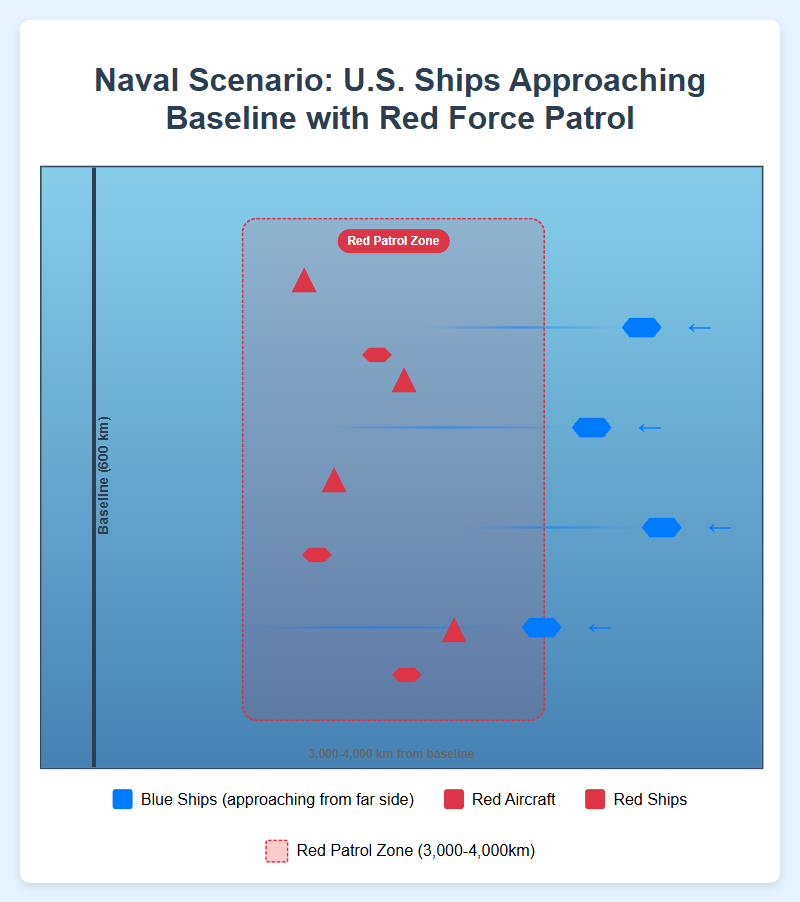
\includegraphics[width=\textwidth]{diagram.png}
	\caption{U.S. ships enter from far side and move towards baseline}
\end{figure}

\section{Agent Model}
The simulation uses an agent-based model as described in the Program Description (see Overleaf.tex):
\begin{itemize}
	\item \textbf{U.S. Ships:} Destroyers and aircraft carriers, modeled in three formations.
	\item \textbf{Chinese UAVs and Fishing Boats:} Patrol agents assigned missions and detection algorithms per Overleaf.tex.
	\item \textbf{Detection:} Based on sensor effectiveness, patrol patterns, and agent interactions. No combat occurs.
\end{itemize}

\section{Simulation Methodology}
\begin{itemize}
	\item Monte Carlo simulation: Randomized agent placement, movement, and detection events.
	\item Each run simulates U.S. ships entering the area and Chinese agents patrolling.
	\item Detection events are logged; time to first detection is recorded for each scenario.
	\item Repeat for all combinations of patrol density and U.S. force composition.
\end{itemize}

\section{Output Requirements}
\subsection{Detection Time Matrix}
The output is a table showing the median time to detection (in hours) for each combination of Chinese patrol density and U.S. force composition.

\begin{table}[H]
	\centering
	\begin{tabular}{|c|c|c|c|}
		\hline
		\multirow{2}{*}{\makecell{\textbf{Chinese} \\ \textbf{Patrol Density}}} & \multicolumn{3}{c|}{\makecell{\textbf{U.S. Force} \\ \textbf{Composition}}} \\
		\cline{2-4}
		& \makecell{\textbf{Single} \\ \textbf{Destroyer}} & \makecell{\textbf{Multiple} \\ \textbf{Destroyers}} & \makecell{\textbf{Destroyers} \\ \textbf{+ Carrier}} \\
		\hline
		\textbf{10\%} & 95\% & 85\% & 75\% \\
		\hline
		\textbf{25\%} & 80\% & 70\% & 60\% \\
		\hline
		\textbf{50\%} & 65\% & 55\% & 45\% \\
		\hline
		\textbf{75\%} & 50\% & 35\% & 20\% \\
		\hline
	\end{tabular}
	\caption{Median Time to Detection (Monte Carlo Results)}
\end{table}

\section{References}
\begin{itemize}
	\item Agent-based model and mission assignment: See Overleaf.tex
	\item Paper structure and analysis: See DraftManuscript.tex
\end{itemize}

\end{document}
